\documentclass{beamer}
%
% Choose how your presentation looks.
%
% For more themes, color themes and font themes, see:
% http://deic.uab.es/~iblanes/beamer_gallery/index_by_theme.html
%
\mode<presentation>
{
  \usetheme{Warsaw}      % or try Darmstadt, Madrid, Warsaw, ...
  \usecolortheme{default}
  \usepackage{beamerthemesplit}% or try albatross, beaver, crane, ...
  \usefonttheme{structurebold}  % or try serif, structurebold, ...
  \setbeamertemplate{navigation symbols}{}
  \setbeamertemplate{caption}[numbered]
  
} 

\usepackage[english]{babel}
\usepackage[utf8x]{inputenc}
\usepackage{amsmath,amssymb}
\usepackage{graphicx} 
\logo{
\includegraphics[height=0.75cm]{images/Logo_Universita_Milano-Bicocca.jpg}}
\title[Schema-Linking \hspace{0.5cm}\insertframenumber/\inserttotalframenumber]{Schema Linking}
\author{Juan Carlos Rosito Cuellar}
\institute{Universita' degli studi di Milano-Bicocca}
\date{16-4-2019}

\usepackage{caption}
\DeclareCaptionFont{xxviii}{\fontsize{7}{7}\selectfont}
\captionsetup{font=xxviii}
\newcommand\Fontvi{\fontsize{6}{9}\selectfont}

\begin{document}


\begin{frame}
	\titlepage
\end{frame}


%\section{Introduction}

\begin{frame}{objectives}
  \begin{itemize}
	\item Make a recommendation of schema semantical annotation and the schema linking of a table.
    \begin{itemize}
		\item Fetch and preprocess the headers of the web table.
		\item Make a surrogate model that can annotate all possible entities of each header, within different ontology’s entities.
		\item Get all the possible decision trees that comprise all the possible entities of the web table.
		\item Get the unique Entities, types and relationships that maximize the similarity of the Web table.
		\item Considerate how the knowledge graph evolves in time
	\end{itemize}
    
  \end{itemize}

\end{frame}

\begin{frame}{Introduction}
  \begin{itemize}
    \item Query Input
    \item Recommender of Vocabulary Term
    \begin{itemize}
		\item Features for ranking
		\item Learning to Ranking
	\end{itemize}
    \item Query Output
  \end{itemize}
  \begin{figure}
	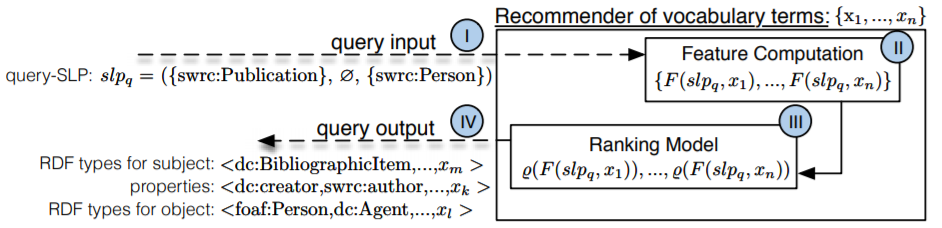
\includegraphics[width=8cm]{images/schema-queryinput.png}
	\caption{\label{fig:your-figure1}Schema of the process of the query}
  \end{figure}
\end{frame}

\begin{frame}{Introduction: Definitions}
  	\begin{figure}
		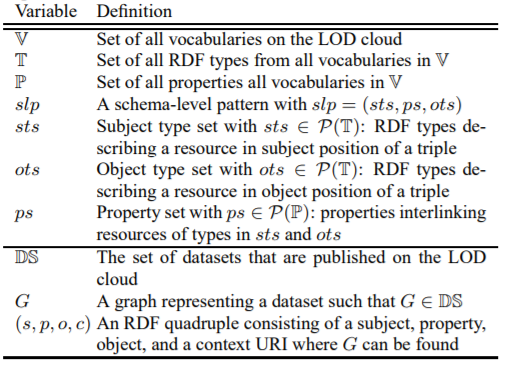
\includegraphics[width=8cm]{images/definition-slp.png}
		\caption{\label{fig:your-figure2} Tabular overview of the variables}
	\end{figure}
\end{frame}

\begin{frame}{Introduction: }
	\begin{figure}
		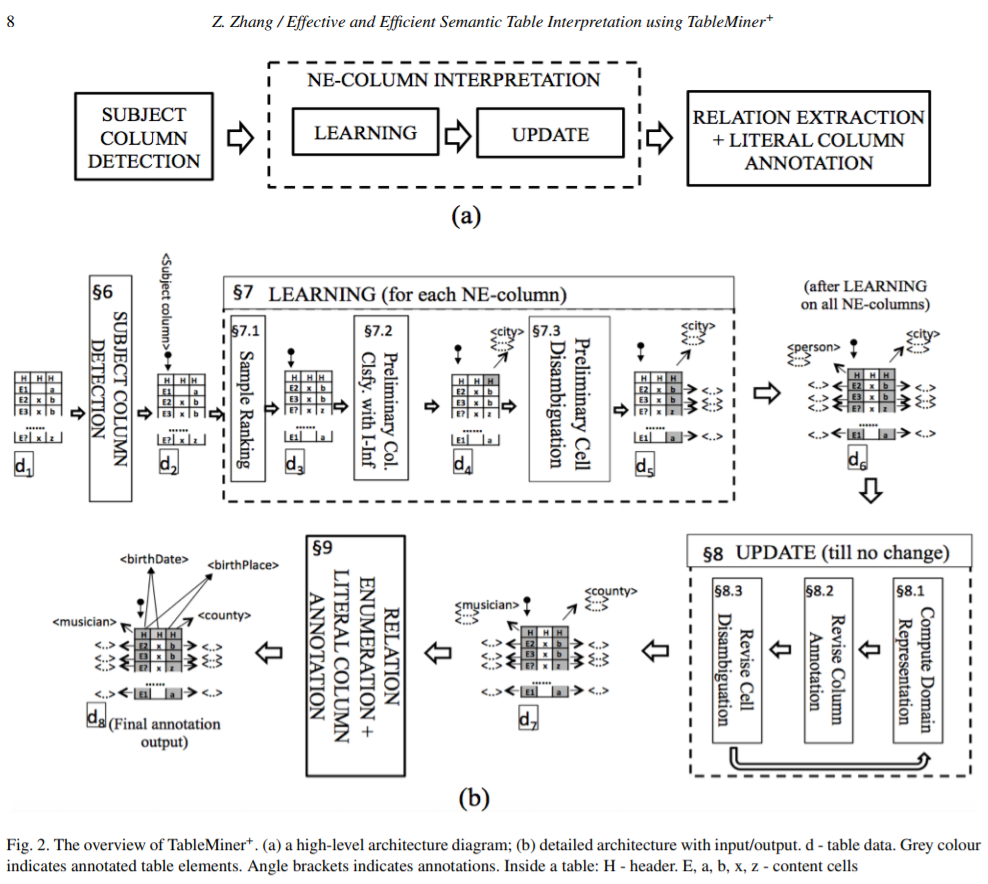
\includegraphics[width=8cm]{images/TableMiner.png}
		\caption{\label{fig:your-figure2} TableMiner design by Z.Zhang}
	\end{figure}
\end{frame}

\begin{frame}{Introduction}
%   \begin{itemize}
%     \item The study that is taken as a reference is “Mapas de Pobreza en Guatemala al 2002” by the National Institute of statistics (INE) of Guatemala. 
%     \item In this study the poverty is taken as a generalized poverty, which take into account the living standard of a person.
%     \item url: \url{http://fadep.org/wp-content/uploads/2016/10/D-5_MAPAS_DE_POBREZA_GUA_2002.pdf}
%   \end{itemize}
\end{frame}

\begin{frame}{Introduction}
%   \begin{figure}
% 		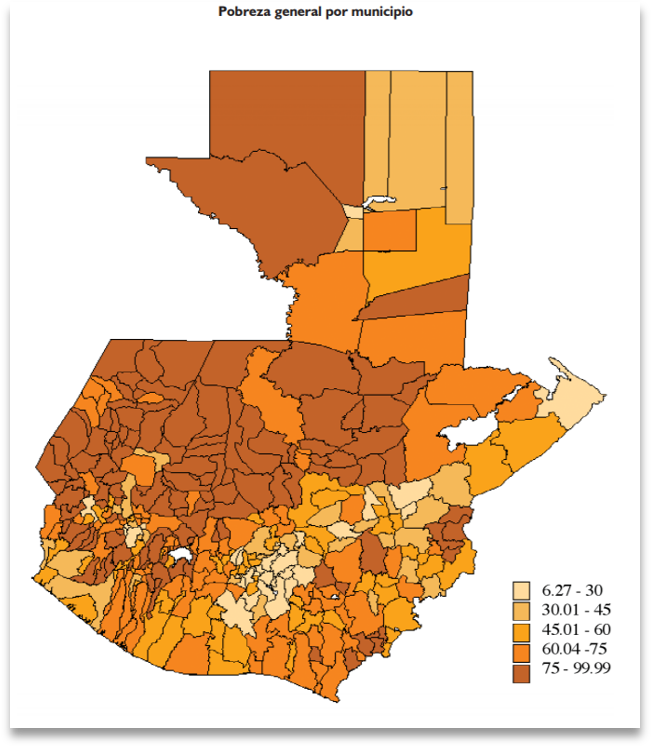
\includegraphics[width=5cm]{images/fig3-map.png}
% 		\caption{\label{fig:your-figure3}Guatemala State Map with a color scale of the generalized poverty}
% 	\end{figure}
\end{frame}

\begin{frame}{Dataset ABSTAT and ontologies}
	% \begin{itemize}
	% 	\item The Data is define in tree modules, the living conditions at the residence, the conditions of each house/apartment/room inside the residence, and finally the characteristics of each person that lives in each residence.
	% \end{itemize}
	% \begin{figure}
	% 	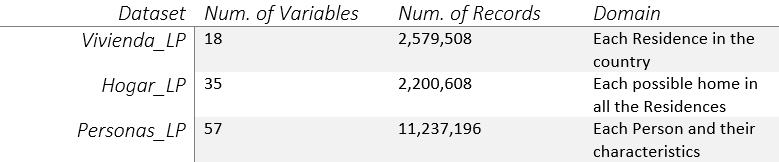
\includegraphics[width=9cm]{images/alldataset.png}
	% 	\caption{\label{fig:alldataset}Datasets taking into consideration in order to make the analysis}
	% \end{figure}
	% \begin{figure}
	% 	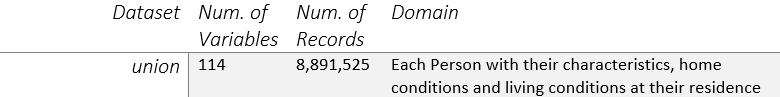
\includegraphics[width=9cm]{images/uniondataset.png}
	% 	\caption{\label{fig:uniondataset}Resulting dataset of the union of Vivienda\_LP, Hogar\_LP and Personas\_LP; filtering records}
	% \end{figure}
\end{frame}

% \begin{frame}{Poverty Index Creation: MPI Aspects }
% 	\begin{itemize}
% 		\item The variables of the Datasets has been measured and has been grouped by the aspects of the MPI of Oxford.
% 	\end{itemize}
% 	\begin{figure}
% 		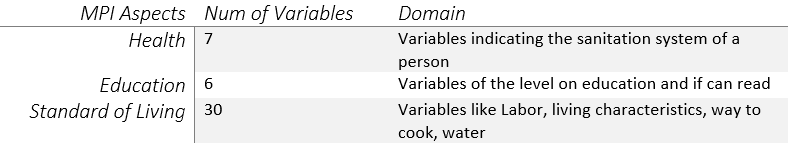
\includegraphics[width=9cm]{images/indexvariables.png}
% 		\caption{\label{fig:indexvariables}Variables took into consideration by the aspects of the MPI created, and the characteristics that the variables have}
% 	\end{figure}
% \end{frame}

% \begin{frame}{Poverty Index Creation: Filtering}
% 	\begin{itemize}
% 		\item Each Variable taken into consideration has effects on the selected data and this lead to some records to be non applicable.
% 		\begin{itemize}
% 			\item Health - the selected data requires that the residence is actually being inhabited by a person and is not a store 
% 			\item Education - the selected data requires that the person been interviewed has more than 6 years old
% 			\item Living - all the persons that satisfy the requirements of Health and Education have the living data
% 		\end{itemize}
% 	\end{itemize}
% \end{frame}

% \begin{frame}{Poverty Index Creation: Result}
% 	\begin{itemize}
% 		\item The resulting dataset has been done by filtering only the variables that were involved on the Multidimensional Poverty Index (MPI) created, and filtering only the records that applied to MPI variables.
% 	\end{itemize}
% 	\begin{figure}
% 		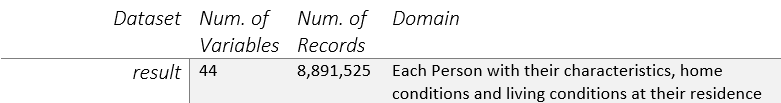
\includegraphics[width=9cm]{images/resultdataset.png}
% 		\caption{\label{fig:resultdataset}Resulting dataset of the union of Vivienda\_LP, Hogar\_LP and Personas\_LP; filtering variables and records}
% 	\end{figure}
% \end{frame}

% \begin{frame}{Poverty Index Comparison - 1}
%   \begin{itemize}
%     \item The metric that it takes as comparison is the index general poverty of the Guatemalan study by INE, that also seek to measure the poverty not only by the income but by the aspects of living of a person. 
%   \end{itemize}
% \end{frame}


% \begin{frame}{Poverty Index Comparison - 2}
%   \begin{figure}
% 		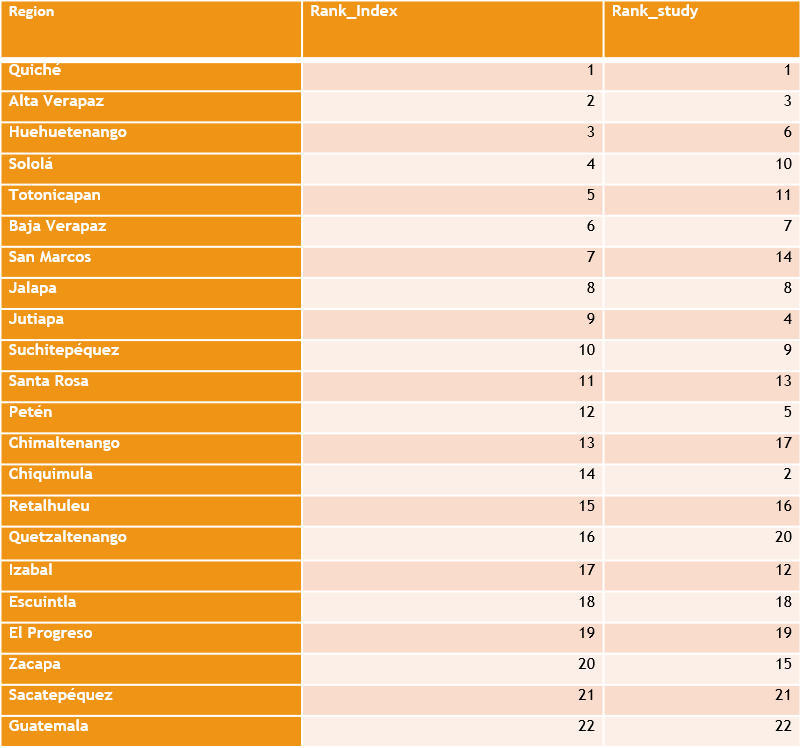
\includegraphics[width=6.5cm]{images/fig4-IndexComp.png}
% 		\caption{\label{fig:your-figure4}Index Table comparison, where Rank\_index is the rank of the generated index with the MPI metrics. The Rank\_study is the rank of the index of Generalized Poverty by the Guatemala Study}
% 	\end{figure}
% \end{frame}

% \begin{frame}{Poverty Index Comparison - 3}
%   \begin{itemize}
%     \item The comparison was made with the paired difference test of “Wilcoxon Signed-Rank Test”.
%     \item The result is that the null hypothesis can’t be refuted, where H0: is that the difference between the pairs follows a symmetric distribution around zero, whit a 0.05 of significance level. With a p-value = 0.8155. So we can't prove that they are different, making a well comparison of the index.
%   \end{itemize}
% \end{frame}

% \begin{frame}{Classification Trees: Introducction - 1}
% 	\begin{figure}
% 		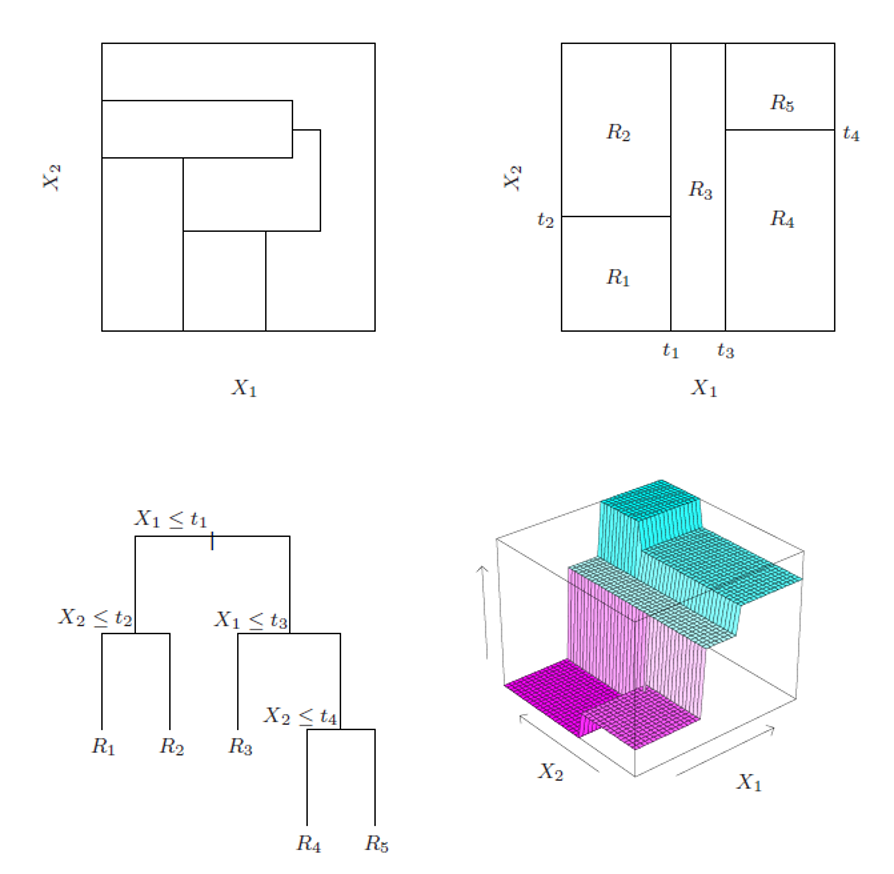
\includegraphics[width=5cm]{images/fig5-decisiontrees.png}
% 		\caption{\label{fig:dtintro} Rerpresents graphicly the regions of a classification tree}
% 	\end{figure}
% \end{frame}

% \begin{frame}{Classification Trees: Introducction - 2}\Fontvi
% 	$$\begin{array}{c}$$
% 	{Getting\ as\ a\ response\ variable\ Y\ and\ p\ explicative\ variables\ as\ X\ }\\{the\ target\ categorical\ variable\ taken\ into\ consideration\ is\ poverty}
% 	\\
% 	{where\ (x_i,y_i)\ goes\ with\ i = 1,2,...,N\ and\ x_i = (x_{i1},x_{i2},...,x_{ip}),\ giving\ N=2\ and\ p=43}\\
% 	{letting\ be\ k\ as\ each\ class\ of\ the\ target\ variable\ and\ m\ as\ identifier\ of\ each\ node.}\\
% 	{In\ a\ node\ m,\ representing\ R_m\ as\ the\ Region}\\
% 	{N_m\ representing\ the\ quantity\ of\ observations\ in\ m}\\\\\\
% 	{It\ can\ be\ said\ that\ the\ proportions\ between\ each\ class\ k\ of}{the\ target\ variable\ in\ each\ node\ m\ can\ be\ represented\ as:}\\
% 	$$
% 		\hat{p}_{mk} = \frac{1}{N_m} ∑_{x_i∈R_m}I(\,y_i = k)\,
% 	\end{array}
% 	$$
% \end{frame}

% \begin{frame}{Classification Trees: Introducction - 3}\Fontvi
% 	$$
% 	\begin{array}{c}
% 	$${the\ splitting\ rule\ took\ was\ the\ Missclassification\ Error,\ where\ can\ be:}\\$$
% 	$${Missclassification\ error:}$$\\
% 	$${Gini\ index: }$$\\
% 	$${Cross-entropy\ of\ deviance:}$$
% 	\end{array}
% 	\begin{array}{c}
% 		\frac{1}{N_m} 		
% 			∑_{i∈R_m}I(\,y_i≠k(\,m)\,)\,  =
% 			1-\hat{p}_{mk(\,m)\,};
% 		$$\\$$
% 			∑_{k≠k'}\hat{p}_{mk}\hat{p}_{mk'} =
% 			∑_{k=1}^{K}\hat{p}_{mk}(\,1-\hat{p}_{mk})\,;
% 		$$\\$$
% 		-∑_{k=1}^K\hat{p}_{mk}\log\hat{p}_{mk};
% 	\end{array}
% 	$$
% \end{frame}



% \begin{frame}{Classification Trees: Introducction - 2}
% 	\begin{figure}
% 		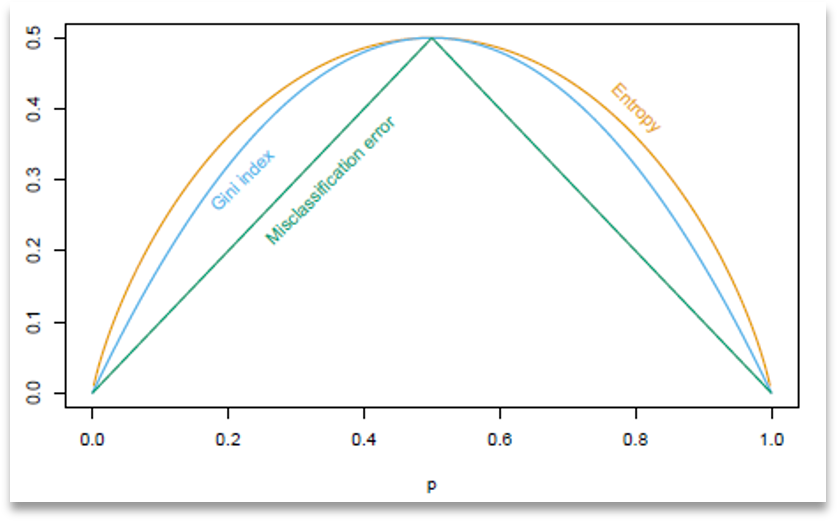
\includegraphics[width=5cm]{images/fig6-dtimpurity.png}
% 		\caption{\label{fig:} Shows the different spliting rules of the classification tree by the measure of impurity, in the x axis show the proportions of the binary target.}
% 	\end{figure}
% \end{frame}


% \begin{frame}{Classification Trees: Result - 1}
% 	\begin{figure}
% 		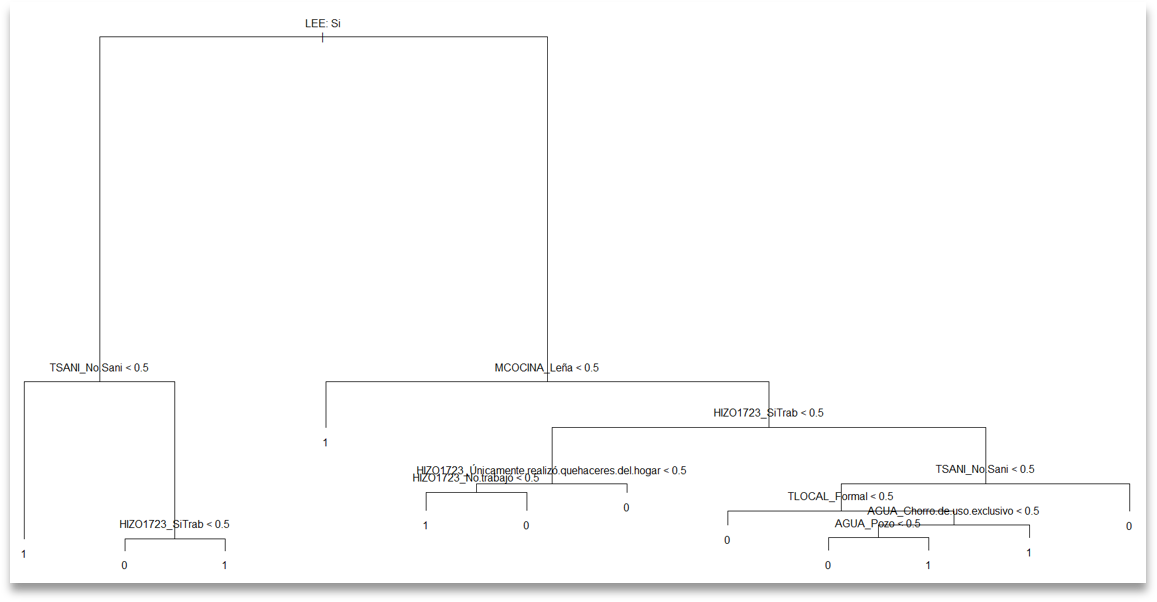
\includegraphics[width=10cm]{images/fig7-dtresult.png}
% 		\caption{\label{fig:dtresult} show the resultant tree of the dichotomous target variable  and the most significant variables}
% 	\end{figure}
% \end{frame}


% \begin{frame}{Classification Trees: Result - 2}
% 	\begin{figure}
% 		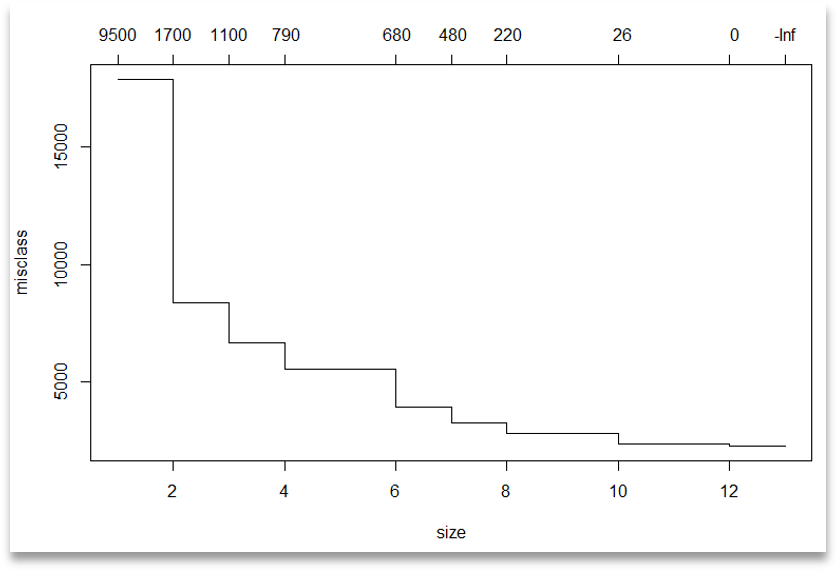
\includegraphics[width=8cm]{images/fig8-dtmissclas.png}
% 		\caption{\label{fig:dtmissclas} Missclassification rate of the prediction by the resultant model of the training of the Classification tree}
% 	\end{figure}
% \end{frame}


% \begin{frame}{LDA (Linear Discrimant Analysis): Introducction - 1}
% 	\begin{figure}
% 		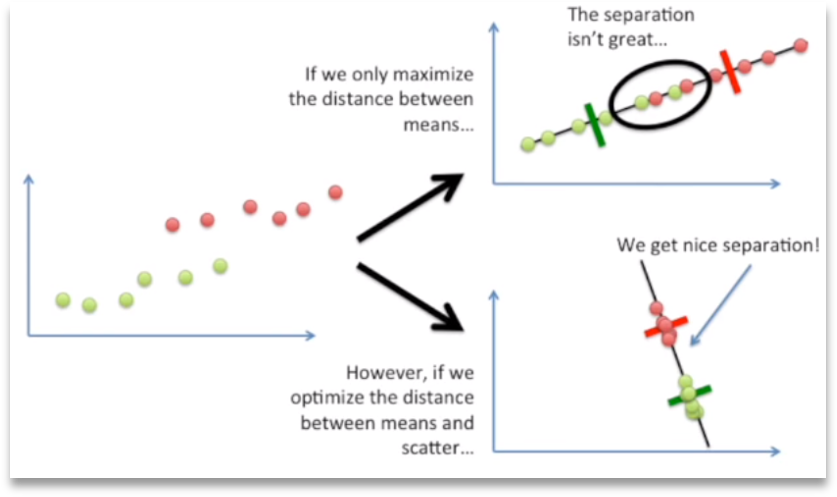
\includegraphics[width=8cm]{images/ldaintro.png}
% 		\caption{\label{fig:ldaintro} The Linear Discriminant Analysis tray to maximize the eucledean distance between groups separation and minimize the variation of each group}
% 	\end{figure}
% \end{frame}

% \begin{frame}{LDA: Introduction - 2}\Fontvi
% 	$$
% 	\begin{array}{c}
% 		$$
% 		{Given\ f_k(x)\ the\ class-conditional\ density\\\ of\ X\ in\ class\ G=k\ and\ letting\ \pi_k\ be\ the\ prior\ probability\ of\ class\ k,\\
% 		Supposing\ that\ each\ class\ density\ is\ modeled\\\ by\ a\ multivariate\ Gaussian,\ the\ discriminant\ function\ is:}\\
% 		$$
% 		\delta_k(x)=x^T∑^{-1}\mu_k-\frac{1}{2}\mu_k^T∑^{-1}\mu_k+\log\pi_k;
% 		$$\\
% 		$$
% 		\hat{ \pi }_k=\frac{N_k}{N},\ where\ N_k\ is\ the\ number\ of\ class-k\ observations;
% 		$$\\
% 		$$
% 		\hat{\mu}_k = ∑_{g_i = k}x_i/N_k
% 		$$\\
% 		$$ 
% 		$$\\{supposing\ that:}
% 		$$
% 		∑_k=∑∀k;
% 		$${where\ the\ target\ variable\ poverty\ is\ categorical\ having\ 2\ classes,\ 0\ or\ 1}\\
% 		$$
% 	\end{array}
% 	$$
% \end{frame}


% \begin{frame}{LDA: Result - 1}
% 	\begin{figure}
% 		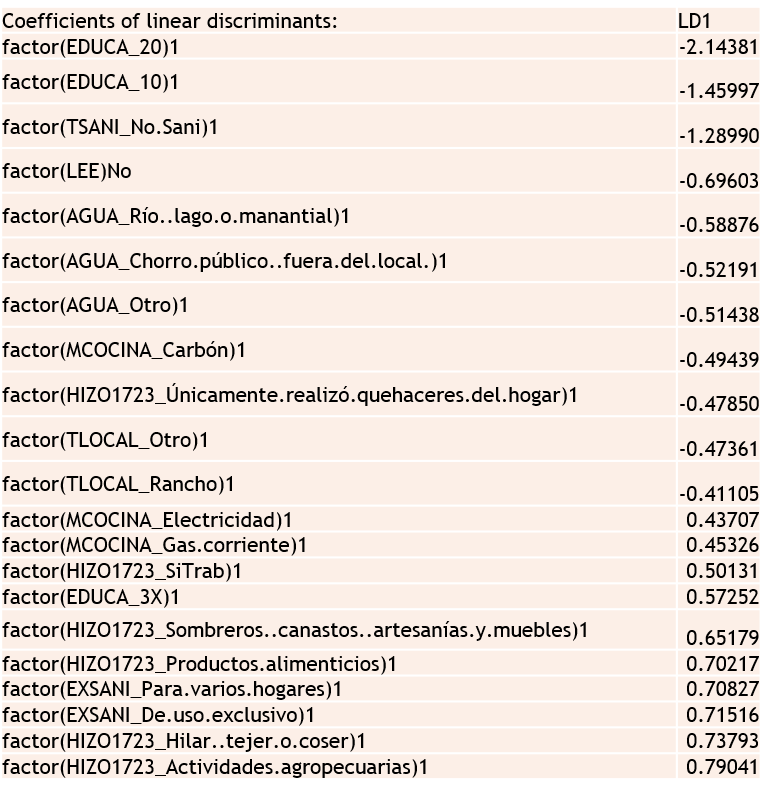
\includegraphics[width=6cm]{images/ldamostvars.png}
% 		\caption{\label{fig:ldamostvars} The most significant variables that separate better the groups if a person is poor or not}
% 	\end{figure}
% \end{frame}



% \begin{frame}{LDA: Result - 2}
% 	\begin{figure}
% 		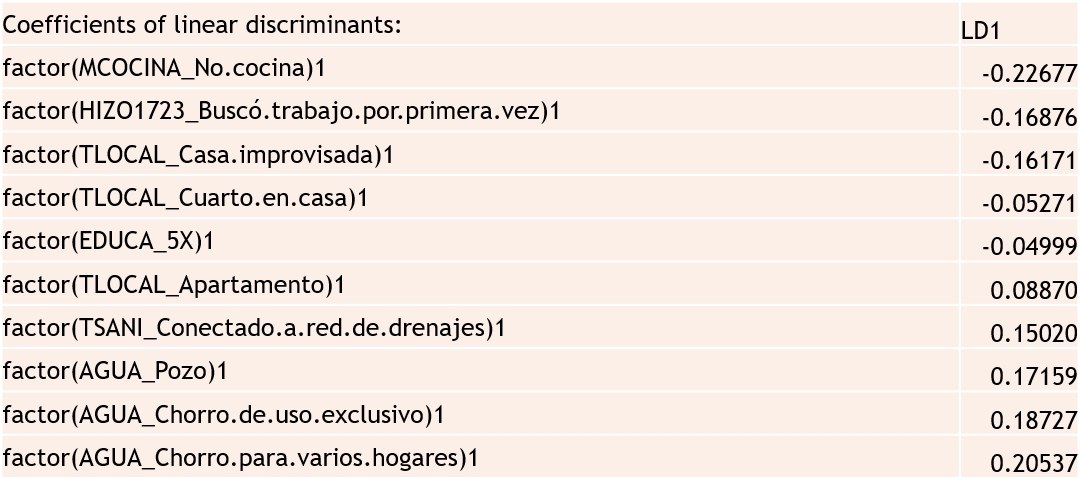
\includegraphics[width=7cm]{images/ldalessvar.png}
% 		\caption{\label{fig:ldalessvar} The less significant variables that separate better the groups if a person is poor or not}
% 	\end{figure}
% \end{frame}



% \begin{frame}{LDA: Result - 3}
% 	\begin{figure}
% 		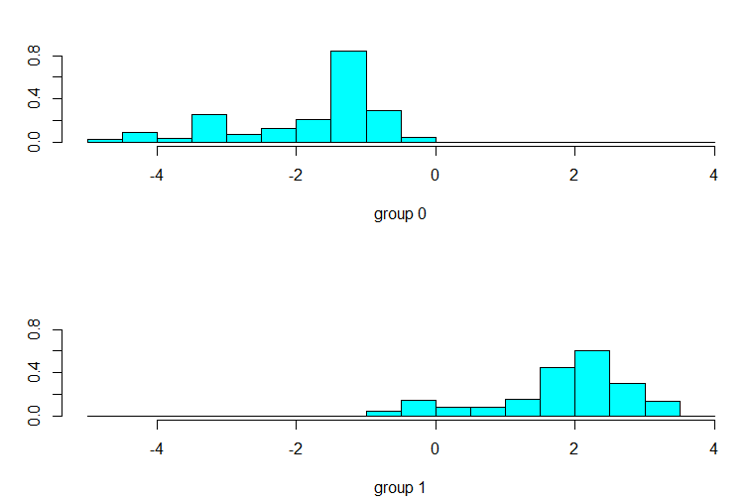
\includegraphics[width=8cm]{images/ldaresult.png}
% 		\caption{\label{fig:ldaresult} Histogram of the quantity of variables that separate each group, the group 0 determines if a person is poor and the group 1 if not}
% 	\end{figure}
% \end{frame}





\begin{frame}{Conclusion}
	\begin{itemize}
		\item 
	\end{itemize}
\end{frame}


\end{document}
